\documentclass[10pt,a4paper,twoside]{article}
\usepackage[T1]{fontenc}
\usepackage[utf8]{inputenc}
\usepackage[brazil]{babel}
% \usepackage{amsmath}
% \usepackage{amsfonts}
% \usepackage{amssymb}
\usepackage{graphicx}
\usepackage{float}
\usepackage[most]{tcolorbox}
\usepackage{titlesec}
\usepackage{lmodern}
\usepackage{geometry}
\usepackage{hyperref}
\geometry{margin=1in}
\renewcommand{\familydefault}{\sfdefault}

\titleformat{\section}
  {\normalfont\Large\bfseries\sffamily}{\thesection}{1em}{}

\providecommand{\tightlist}{%
  \setlength{\itemsep}{0pt}\setlength{\parskip}{0pt}}

\newcounter{grammarbox}[section]
\renewcommand{\thegrammarbox}{\thesection.\arabic{grammarbox}}
\makeatletter
\newtcolorbox{grammarbox}[2][]{
  colback=gray!10,
  colframe=black!70,
  fonttitle=\bfseries,
  coltitle=white,
  left=2mm,
  right=2mm,
  top=1mm,
  bottom=1mm,
  arc=4pt,
  boxrule=0.7pt,
  enhanced,
  attach boxed title to top left={yshift=-2mm, xshift=2mm},
  boxed title style={
    colback=black!60,
    colframe=black!60,
    rounded corners,
    boxrule=0pt,
    left=3pt,
    right=3pt,
    top=3pt,
    bottom=3pt,
  },
  before upper={
    \phantomsection
    \refstepcounter{grammarbox}
    \def\@currentlabelname{#2}
    \label{#1}
  },
  title={#2}
}
\makeatother

\title{PascalM The Most Better BNF}
\author{Murilo Henrique Alves}
\date{2025-05-30}

\begin{document}
\maketitle

\section{Introdução}
A gramática PascalM é uma evolução da gramática padrão ISO do Pascal.
Ela aprimora a definição de tipos estruturados, adiciona suporte mais claro
para registros, arrays e variantes, além de incorporar uma definição mais
rígida e completa para expressões compostas, operadores e listas de parâmetros.

\section{Regras da Gramática}

\textbf{program:}

\begin{figure}[H]
\centering

\includegraphics{diagram/program.pdf}

\end{figure}

\begin{grammarbox}[grammar:program]{program}
\vspace{0.5em}
program  ::= 'program' identifier program\_headingopt ';' block '.'
\end{grammarbox}

\textbf{program\_headingopt:}

\begin{figure}[H]
\centering
\includegraphics{diagram/program_headingopt.pdf}

\end{figure}

\begin{grammarbox}[grammar:program_headingopt]{program\_headingopt}
\vspace{0.5em}
program\_headingopt
         ::= ( '(' identifier\_list ')' )?
\end{grammarbox}

referenced by:

\begin{itemize}
\tightlist
\item
  \nameref{grammar:program}
\end{itemize}

\textbf{identifier\_list:}

\begin{figure}[H]
\centering
\includegraphics{diagram/identifier_list.pdf}

\end{figure}

\begin{grammarbox}[grammar:identifier_list]{identifier\_list}
\vspace{0.5em}
identifier\_list
         ::= identifier ( ',' identifier )*
\end{grammarbox}

referenced by:

\begin{itemize}
\tightlist
\item
  \nameref{grammar:program_headingopt}
\item
  \nameref{grammar:simple_type}
\end{itemize}

\textbf{block:}

\begin{figure}[H]
\centering
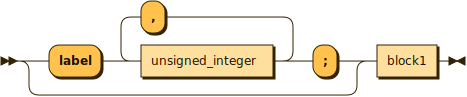
\includegraphics{diagram/block.pdf}

\end{figure}

\begin{grammarbox}[grammar:block]{block}
\vspace{0.5em}
block    ::= ( 'label' unsigned\_integer ( ',' unsigned\_integer )* ';' )? block1
\end{grammarbox}

referenced by:

\begin{itemize}
\tightlist
\item
  \nameref{grammar:block_or_forward}
\item
  \nameref{grammar:program}
\end{itemize}

\textbf{block1:}

\begin{figure}[H]
\centering
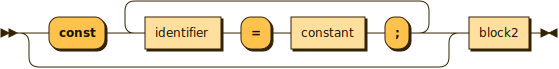
\includegraphics{diagram/block1.pdf}

\end{figure}

\begin{grammarbox}[grammar:block1]{block1}
\vspace{0.5em}
block1   ::= ( 'const' ( identifier '=' constant ';' )+ )? block2
\end{grammarbox}

referenced by:

\begin{itemize}
\tightlist
\item
  \nameref{grammar:block}
\end{itemize}

\textbf{block2:}

\begin{figure}[H]
\centering
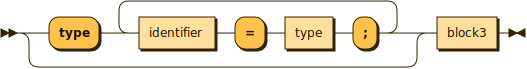
\includegraphics{diagram/block2.pdf}

\end{figure}

\begin{grammarbox}[grammar:block2]{block2}
\vspace{0.5em}
block2   ::= ( 'type' ( identifier '=' type ';' )+ )? block3
\end{grammarbox}

referenced by:

\begin{itemize}
\tightlist
\item
  \nameref{grammar:block1}
\end{itemize}

\textbf{block3:}

\begin{figure}[H]
\centering
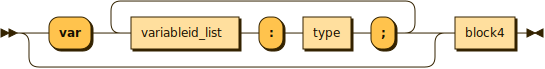
\includegraphics{diagram/block3.pdf}

\end{figure}

\begin{grammarbox}[grammar:block3]{block3}
\vspace{0.5em}
block3   ::= ( 'var' ( variableid\_list ':' type ';' )+ )? block4
\end{grammarbox}

referenced by:

\begin{itemize}
\tightlist
\item
  \nameref{grammar:block2}
\end{itemize}

\textbf{block4:}

\begin{figure}[H]
\centering
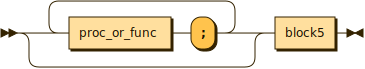
\includegraphics{diagram/block4.pdf}

\end{figure}

\begin{grammarbox}[grammar:block4]{block4}
\vspace{0.5em}
block4   ::= ( proc\_or\_func ';' )* block5
\end{grammarbox}

referenced by:

\begin{itemize}
\tightlist
\item
  \nameref{grammar:block3}
\end{itemize}

\textbf{block5:}

\begin{figure}[H]
\centering
\includegraphics{diagram/block5.pdf}

\end{figure}

\begin{grammarbox}[grammar:block5]{block5}
\vspace{0.5em}
block5   ::= 'begin' statement\_list 'end'
\end{grammarbox}

referenced by:

\begin{itemize}
\tightlist
\item
  \nameref{grammar:block4}
\end{itemize}

\textbf{variableid\_list:}

\begin{figure}[H]
\centering
\includegraphics{diagram/variableid_list.pdf}

\end{figure}

\begin{grammarbox}[grammar:variableid_list]{variableid\_list}
\ttfamily
\vspace*{0.5em}
variableid\_list :== identifier ( ',' identifier )*
\end{grammarbox}

referenced by:

\begin{itemize}
\tightlist
\item
  \nameref{grammar:block3}
\end{itemize}

\textbf{constant:}

\begin{figure}[H]
\centering
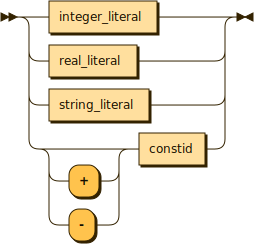
\includegraphics{diagram/constant.pdf}
\end{figure}

\begin{grammarbox}[grammar:constant]{constant}
\ttfamily
\vspace*{0.5em}
constant ::= \\
    integer\_literal \\
  \hspace*{1.5em} | real\_literal \\
  \hspace*{1.5em} | string\_literal \\
  \hspace*{1.5em} | ( '+' | '-' )? constid
\end{grammarbox}

referenced by:

\begin{itemize}
\tightlist
\item
  \nameref{grammar:block1}
\item
  \nameref{grammar:case_label_list}
\item
  \nameref{grammar:simple_type}
\end{itemize}

\textbf{type:}

\begin{figure}[H]
\centering
  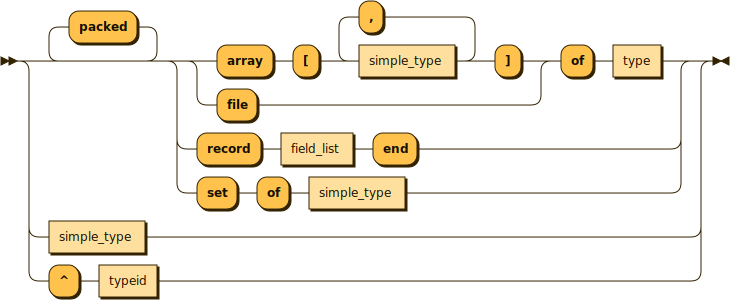
\includegraphics[width=1\textwidth]{diagram/type.pdf}

\end{figure}

\begin{grammarbox}[grammar:type]{type}
\ttfamily
  \vspace*{0.5em}
type ::= simple\_type \\
\hspace*{1.5em} | 'packed'* ( ( 'array' '[' simple\_type ( ',' simple\_type )* ']' | 'file' ) 'of' type | 'record' field\_list 'end' | 'set' 'of' simple\_type ) \\
\hspace*{1.5em} | '\^{}' typeid
\end{grammarbox}

referenced by:

\begin{itemize}
\tightlist
\item
  \nameref{grammar:block2}
\item
  \nameref{grammar:block3}
\item
  \nameref{grammar:record_field}
\item
  \nameref{grammar:type}
\end{itemize}

\textbf{simple\_type:}

\begin{figure}[H]
\centering
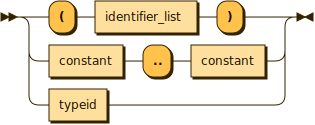
\includegraphics{diagram/simple_type.pdf}

\end{figure}

\begin{grammarbox}[grammar:simple_type]{simple\_type}
\vspace{0.5em}
simple\_type
         ::= '(' identifier\_list ')'
           | constant '..' constant
           | typeid
\end{grammarbox}

referenced by:

\begin{itemize}
\tightlist
\item
  \nameref{grammar:type}
\end{itemize}

\textbf{field\_list:}

\begin{figure}[H]
\centering
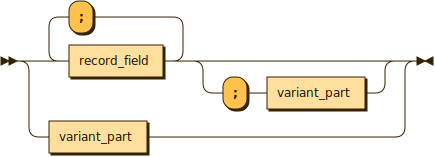
\includegraphics{diagram/field_list.pdf}

\end{figure}

\begin{grammarbox}[grammar:field_list]{field\_list}
\vspace{0.5em}
 field\_list
         ::= record\_field ( ';' record\_field )* ( ';' variant\_part )?
           | variant\_part
\end{grammarbox}

referenced by:

\begin{itemize}
\tightlist
\item
  \nameref{grammar:type}
\item
  \nameref{grammar:variant}
\end{itemize}

\textbf{record\_field:}

\begin{figure}[H]
\centering
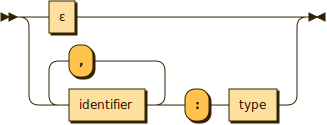
\includegraphics{diagram/record_field.pdf}

\end{figure}

\begin{grammarbox}[grammar:record_field]{record\_field}
\vspace{0.5em}
record\_field
         ::= $\varepsilon$
           | identifier ( ',' identifier )* ':' type
\end{grammarbox}

referenced by:

\begin{itemize}
\tightlist
\item
  \nameref{grammar:field_list}
\end{itemize}

\textbf{variant\_part:}

\begin{figure}[H]
\centering
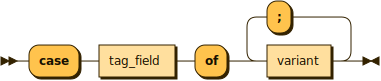
\includegraphics{diagram/variant_part.pdf}

\end{figure}

\begin{grammarbox}[grammar:variant_part]{variant\_part}
\vspace{0.5em}
variant\_part
         ::= 'case' tag\_field 'of' variant ( ';' variant )*
\end{grammarbox}

referenced by:

\begin{itemize}
\tightlist
\item
  \nameref{grammar:field_list}
\end{itemize}

\textbf{tag\_field:}

\begin{figure}[H]
\centering
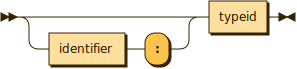
\includegraphics{diagram/tag_field.pdf}

\end{figure}

\begin{grammarbox}[grammar:tag_field]{tag\_field}
\vspace{0.5em}
tag\_field
         ::= ( identifier ':' )? typeid
\end{grammarbox}

referenced by:

\begin{itemize}
\tightlist
\item
  \nameref{grammar:variant_part}
\end{itemize}

\textbf{variant:}

\begin{figure}[H]
\centering
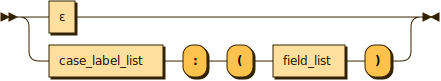
\includegraphics{diagram/variant.pdf}

\end{figure}

\begin{grammarbox}[grammar:variant]{variant}
\vspace{0.5em}
variant  ::= $\varepsilon$
           | case\_label\_list ':' '(' field\_list ')'
\end{grammarbox}

referenced by:

\begin{itemize}
\tightlist
\item
  \nameref{grammar:variant_part}
\end{itemize}

\textbf{case\_label\_list:}

\begin{figure}[H]
\centering
\includegraphics{diagram/case_label_list.pdf}

\end{figure}

\begin{grammarbox}[grammar:case_label_list]{case\_label\_list}
\vspace{0.5em}
case\_label\_list
         ::= constant ( ',' constant )*
\end{grammarbox}

referenced by:

\begin{itemize}
\tightlist
\item
  \nameref{grammar:case_element}
\item
  \nameref{grammar:variant}
\end{itemize}

\textbf{proc\_or\_func:}

\begin{figure}[H]
\centering
  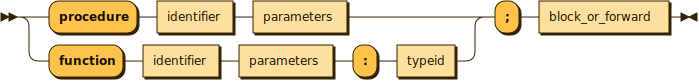
\includegraphics[width=1\textwidth]{diagram/proc_or_func.pdf}

\end{figure}

\begin{grammarbox}[grammar:proc_or_func]{proc\_or\_func}
\vspace{0.5em}
proc\_or\_func
         ::= ( 'procedure' identifier parameters | 'function' identifier parameters ':' typeid ) ';' block\_or\_forward
\end{grammarbox}

referenced by:

\begin{itemize}
\tightlist
\item
  \nameref{grammar:block4}
\end{itemize}

\textbf{block\_or\_forward:}

\begin{figure}[H]
\centering
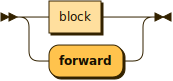
\includegraphics{diagram/block_or_forward.pdf}

\end{figure}

\begin{grammarbox}[grammar:block_or_forward]{block\_or\_forward}
\vspace{0.5em}
block\_or\_forward
         ::= block
           | 'forward'
\end{grammarbox}

referenced by:

\begin{itemize}
\tightlist
\item
  proc\_or\_func
\end{itemize}

\textbf{parameters:}

\begin{figure}[H]
\centering
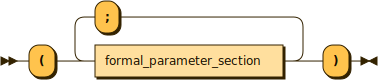
\includegraphics{diagram/parameters.pdf}

\end{figure}

\begin{grammarbox}[grammar:parameters]{parameters}
\vspace{0.5em}
parameters
         ::= '(' formal\_parameter\_section ( ';' formal\_parameter\_section )* ')'
\end{grammarbox}

referenced by:

\begin{itemize}
\tightlist
\item
  \nameref{grammar:formal_parameter_section}
\item
  proc\_or\_func
\end{itemize}

\textbf{formal\_parameter\_section:}

\begin{figure}[H]
\centering
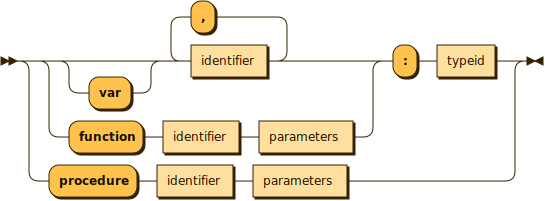
\includegraphics{diagram/formal_parameter_section.pdf}

\end{figure}

\begin{grammarbox}[grammar:formal_parameter_section]{formal\_parameter\_section}
\vspace{0.5em}
formal\_parameter\_section
         ::= ( 'var'? identifier ( ',' identifier )* | 'function' identifier parameters ) ':' typeid
           | 'procedure' identifier parameters
\end{grammarbox}

referenced by:

\begin{itemize}
\tightlist
\item
  \nameref{grammar:parameters}
\end{itemize}

\textbf{statement:}

\begin{figure}[H]
\centering
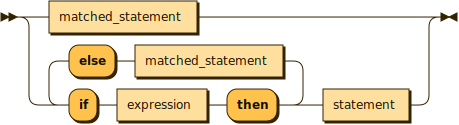
\includegraphics{diagram/statement.pdf}

\end{figure}

\begin{grammarbox}[grammar:statement]{statement}
\vspace{0.5em}
statement
         ::= matched\_statement
           | 'if' expression 'then' ( matched\_statement 'else' 'if' expression 'then' )* statement
\end{grammarbox}

referenced by:

\begin{itemize}
\tightlist
\item
  \nameref{grammar:case_element}
\item
  \nameref{grammar:case_else}
\item
  \nameref{grammar:other_statement}
\item
  \nameref{grammar:statement}
\item
  \nameref{grammar:statement_list}
\end{itemize}

\textbf{matched\_statement:}

\begin{figure}[H]
\centering
  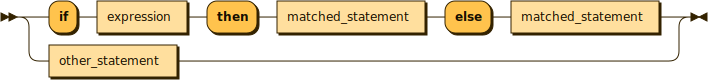
\includegraphics[width=1.0\textwidth]{diagram/matched_statement.pdf}

\end{figure}

\begin{grammarbox}[grammar:matched_statement]{matched\_statement}
\vspace{0.5em}
matched\_statement
         ::= 'if' expression 'then' matched\_statement 'else' matched\_statement
           | other\_statement
\end{grammarbox}

referenced by:

\begin{itemize}
\tightlist
\item
  \nameref{grammar:matched_statement}
\item
  \nameref{grammar:statement}
\end{itemize}

\textbf{other\_statement:}

\begin{figure}[H]
\centering
  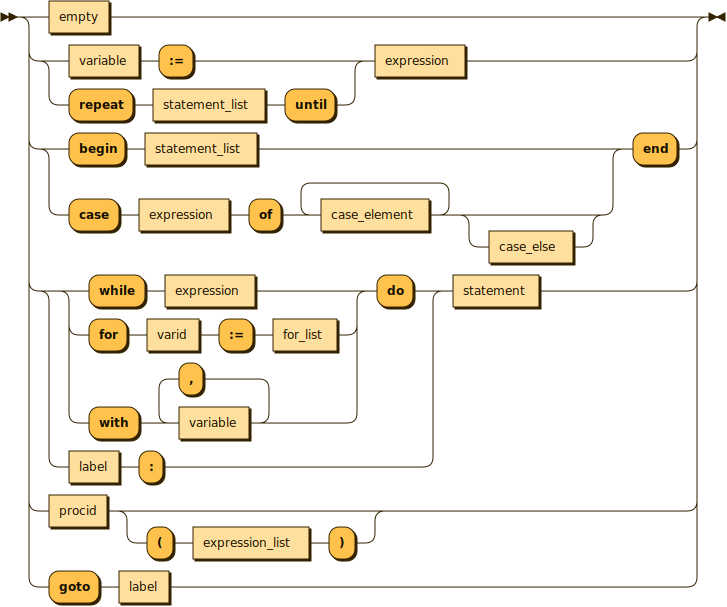
\includegraphics[width=1.0\textwidth]{diagram/other_statement.pdf}

\end{figure}

\begin{grammarbox}[grammar:other_statement]{other\_statement}
\vspace{0.5em}
other\_statement
         ::= empty
           | ( variable ':=' | 'repeat' statement\_list 'until' ) expression
           | ( 'begin' statement\_list | 'case' expression 'of' case\_element+ case\_else? ) 'end'
           | ( ( 'while' expression | 'for' varid ':=' for\_list | 'with' variable ( ',' variable )* ) 'do' | label ':' ) statement
           | procid ( '(' expression\_list ')' )?
           | 'goto' label
\end{grammarbox}

referenced by:

\begin{itemize}
\tightlist
\item
  \nameref{grammar:matched_statement}
\end{itemize}

\textbf{expression:}

\begin{figure}[H]
\centering
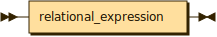
\includegraphics{diagram/expression.pdf}

\end{figure}

\begin{grammarbox}[grammar:expression]{expression}
\vspace{0.5em}
expression
         ::= relational\_expression
\end{grammarbox}

referenced by:

\begin{itemize}
\tightlist
\item
  \nameref{grammar:element}
\item
  \nameref{grammar:expression_list}
\item
  \nameref{grammar:for_list}
\item
  \nameref{grammar:matched_statement}
\item
  \nameref{grammar:other_statement}
\item
  \nameref{grammar:primary_expression}
\item
  \nameref{grammar:statement}
\item
  \nameref{grammar:variable}
\end{itemize}

\textbf{relational\_expression:}

\begin{figure}[H]
\centering
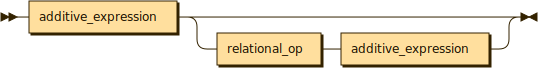
\includegraphics{diagram/relational_expression.pdf}

\end{figure}

\begin{grammarbox}[grammar:relational_expression]{relational\_expression}
\vspace{0.5em}
relational\_expression
         ::= additive\_expression ( relational\_op additive\_expression )?
\end{grammarbox}

referenced by:

\begin{itemize}
\tightlist
\item
  \nameref{grammar:expression}
\end{itemize}

\textbf{additive\_expression:}

\begin{figure}[H]
\centering
\includegraphics{diagram/additive_expression.pdf}

\end{figure}

\begin{grammarbox}[grammar:additive_expression]{additive\_expression}
\vspace{0.5em}
additive\_expression
         ::= multiplicative\_expression ( add\_op multiplicative\_expression )*
\end{grammarbox}

referenced by:

\begin{itemize}
\tightlist
\item
  \nameref{grammar:relational_expression}
\end{itemize}

\textbf{multiplicative\_expression:}

\begin{figure}[H]
\centering
\includegraphics{diagram/multiplicative_expression.pdf}

\end{figure}

\begin{grammarbox}[grammar:multiplicative_expression]{multiplicative\_expression}
\vspace{0.5em}
multiplicative\_expression
         ::= unary\_expression ( mul\_op unary\_expression )*
\end{grammarbox}

referenced by:

\begin{itemize}
\tightlist
\item
  \nameref{grammar:additive_expression}
\end{itemize}

\textbf{unary\_expression:}

\begin{figure}[H]
\centering
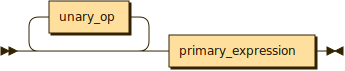
\includegraphics{diagram/unary_expression.pdf}

\end{figure}

\begin{grammarbox}[grammar:unary_expression]{unary\_expression}
\vspace{0.5em}
unary\_expression
         ::= unary\_op* primary\_expression
\end{grammarbox}

referenced by:

\begin{itemize}
\tightlist
\item
  \nameref{grammar:multiplicative_expression}
\end{itemize}

\textbf{primary\_expression:}

\begin{figure}[H]
\centering
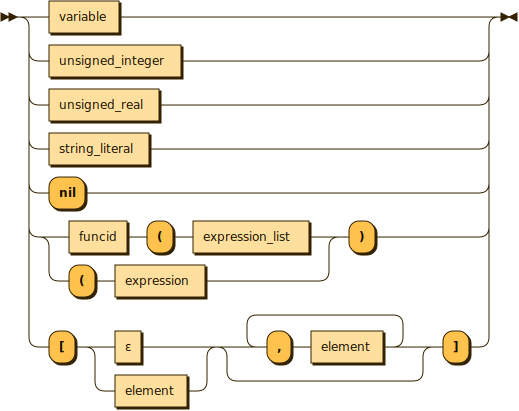
\includegraphics{diagram/primary_expression.pdf}

\end{figure}

\begin{grammarbox}[grammar:primary_expression]{primary\_expression}
\vspace{0.5em}
primary\_expression
         ::= variable
           | unsigned\_integer
           | unsigned\_real
           | string\_literal
           | 'nil'
           | ( funcid '(' expression\_list | '(' expression ) ')'
           | '[' ( $\varepsilon$ | element ) ( ',' element )* ']'
\end{grammarbox}

referenced by:

\begin{itemize}
\tightlist
\item
  \nameref{grammar:unary_expression}
\end{itemize}

\textbf{expression\_list:}

\begin{figure}[H]
\centering
\includegraphics{diagram/expression_list.pdf}

\end{figure}

\begin{grammarbox}[grammar:expression_list]{expression\_list}
\vspace{0.5em}
expression\_list
         ::= expression ( ',' expression )*
\end{grammarbox}

referenced by:

\begin{itemize}
\tightlist
\item
  \nameref{grammar:other_statement}
\item
  \nameref{grammar:primary_expression}
\end{itemize}

\textbf{element:}

\begin{figure}[H]
\centering
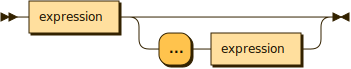
\includegraphics{diagram/element.pdf}

\end{figure}

\begin{grammarbox}[grammar:element]{element}
\vspace{0.5em}
element  ::= expression ( '...' expression )?
\end{grammarbox}

referenced by:

\begin{itemize}
\tightlist
\item
  \nameref{grammar:primary_expression}
\end{itemize}

\textbf{relational\_op:}

\begin{figure}[H]
\centering
\includegraphics{diagram/relational_op.pdf}

\end{figure}

\begin{grammarbox}[grammar:relational_op]{relational\_op}
\vspace{0.5em}
relational\_op
         ::= '<'
           | '<='
           | '='
           | '<>'
           | '>='
           | '>'
\end{grammarbox}

referenced by:

\begin{itemize}
\tightlist
\item
  \nameref{grammar:relational_expression}
\end{itemize}

\textbf{add\_op:}

\begin{figure}[H]
\centering
\includegraphics{diagram/add_op.pdf}

\end{figure}

\begin{grammarbox}[grammar:add_op]{add\_op}
\vspace{0.5em}
add\_op   ::= '+'
           | '-'
           | 'or'
\end{grammarbox}

referenced by:

\begin{itemize}
\tightlist
\item
  \nameref{grammar:additive_expression}
\end{itemize}

\textbf{mul\_op:}

\begin{figure}[H]
\centering
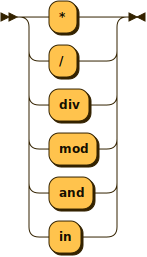
\includegraphics{diagram/mul_op.pdf}

\end{figure}

\begin{grammarbox}[grammar:mul_op]{mul\_op}
\vspace{0.5em}
mul\_op   ::= '*'
           | '/'
           | 'div'
           | 'mod'
           | 'and'
           | 'in'
\end{grammarbox}

referenced by:

\begin{itemize}
\tightlist
\item
  \nameref{grammar:multiplicative_expression}
\end{itemize}

\textbf{unary\_op:}

\begin{figure}[H]
\centering
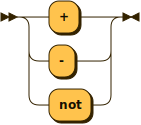
\includegraphics{diagram/unary_op.pdf}

\end{figure}

\begin{grammarbox}[grammar:unary_op]{unary\_op}
\vspace{0.5em}
unary\_op ::= '+'
           | '-'
           | 'not'
\end{grammarbox}

referenced by:

\begin{itemize}
\tightlist
\item
  \nameref{grammar:unary_expression}
\end{itemize}

\textbf{statement\_list:}

\begin{figure}[H]
\centering
\includegraphics{diagram/statement_list.pdf}

\end{figure}

\begin{grammarbox}[grammar:statement_list]{statement\_list}
\vspace{0.5em}
statement\_list
         ::= statement ( ';' statement )*
\end{grammarbox}

referenced by:

\begin{itemize}
\tightlist
\item
  \nameref{grammar:block5}
\item
  \nameref{grammar:other_statement}
\end{itemize}

\textbf{case\_element:}

\begin{figure}[H]
\centering

\includegraphics{diagram/case_element.pdf}

\end{figure}

\begin{grammarbox}[grammar:case_element]{case\_element}
\vspace{0.5em}
case\_element
         ::= case\_label\_list ':' statement ';'
\end{grammarbox}

referenced by:

\begin{itemize}
\tightlist
\item
  \nameref{grammar:other_statement}
\end{itemize}

\textbf{case\_else:}

\begin{figure}[H]
\centering
\includegraphics{diagram/case_else.pdf}

\end{figure}

\begin{grammarbox}[grammar:case_else]{case\_else}
\vspace{0.5em}
case\_else
         ::= 'else' statement ';'
\end{grammarbox}

referenced by:

\begin{itemize}
\tightlist
\item
  \nameref{grammar:other_statement}
\end{itemize}

\textbf{for\_list:}

\begin{figure}[H]
\centering
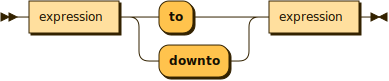
\includegraphics{diagram/for_list.pdf}

\end{figure}

\begin{grammarbox}[grammar:for_list]{for\_list}
\vspace{0.5em}
for\_list ::= expression ( 'to' | 'downto' ) expression
\end{grammarbox}

referenced by:

\begin{itemize}
\tightlist
\item
  \nameref{grammar:other_statement}
\end{itemize}

\textbf{variable:}

\begin{figure}[H]
\centering
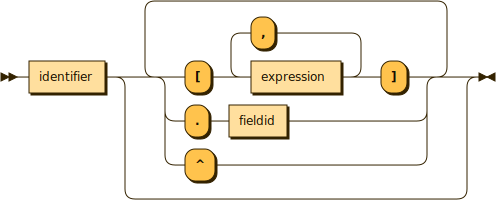
\includegraphics{diagram/variable.pdf}

\end{figure}

\begin{grammarbox}[grammar:variable]{variable}
\vspace{0.5em}
variable ::= identifier ( '[' expression ( ',' expression )* ']' | '.' fieldid | '\^{}' )*
\end{grammarbox}

referenced by:

\begin{itemize}
\tightlist
\item
  \nameref{grammar:other_statement}
\item
  \nameref{grammar:primary_expression}
\end{itemize}

\textbf{identifier:}

\begin{figure}[H]
\centering
\includegraphics{diagram/identifier.pdf}

\end{figure}

\begin{grammarbox}[grammar:identifier]{identifier}
\vspace{0.5em}
identifier
         ::= IDENTIFIER
\end{grammarbox}

referenced by:

\begin{itemize}
\tightlist
\item
  \nameref{grammar:block1}
\item
  \nameref{grammar:block2}
\item
  \nameref{grammar:constid}
\item
  \nameref{grammar:fieldid}
\item
  \nameref{grammar:formal_parameter_section}
\item
  \nameref{grammar:funcid}
\item
  \nameref{grammar:identifier_list}
\item
  \nameref{grammar:proc_or_func}
\item
  \nameref{grammar:procid}
\item
  \nameref{grammar:program}
\item
  \nameref{grammar:record_field}
\item
  \nameref{grammar:tag_field}
\item
  \nameref{grammar:typeid}
\item
  \nameref{grammar:variable}
\item
  \nameref{grammar:variableid_list}
\item
  \nameref{grammar:varid}
\end{itemize}

\textbf{funcid:}

\begin{figure}[H]
\centering
\includegraphics{diagram/funcid.pdf}

\end{figure}

\begin{grammarbox}[grammar:funcid]{funcid}
\vspace{0.5em}
funcid   ::= identifier
\end{grammarbox}

referenced by:

\begin{itemize}
\tightlist
\item
  \nameref{grammar:primary_expression}
\end{itemize}

\textbf{procid:}

\begin{figure}[H]
\centering
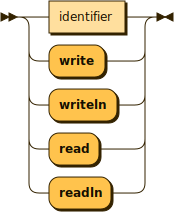
\includegraphics{diagram/procid.pdf}

\end{figure}

\begin{grammarbox}[grammar:procid]{procid}
\vspace{0.5em}
procid   ::= identifier
           | 'write'
           | 'writeln'
           | 'read'
           | 'readln'
\end{grammarbox}

referenced by:

\begin{itemize}
\tightlist
\item
  \nameref{grammar:other_statement}
\end{itemize}

\textbf{varid:}

\begin{figure}[H]
\centering
\includegraphics{diagram/varid.pdf}

\end{figure}

\begin{grammarbox}[grammar:varid]{varid}
\vspace{0.5em}
varid    ::= identifier
\end{grammarbox}

referenced by:

\begin{itemize}
\tightlist
\item
  \nameref{grammar:other_statement}
\end{itemize}

\textbf{fieldid:}

\begin{figure}[H]
\centering
\includegraphics{diagram/fieldid.pdf}

\end{figure}

\begin{grammarbox}[grammar:fieldid]{fieldid}
\vspace{0.5em}
fieldid  ::= identifier
\end{grammarbox}

referenced by:

\begin{itemize}
\tightlist
\item
  \nameref{grammar:variable}
\end{itemize}

\textbf{constid:}

\begin{figure}[H]
\centering
\includegraphics{diagram/constid.pdf}

\end{figure}

\begin{grammarbox}[grammar:constid]{constid}
\vspace{0.5em}
constid  ::= identifier
\end{grammarbox}

referenced by:

\begin{itemize}
\tightlist
\item
  \nameref{grammar:constant}
\end{itemize}

\textbf{typeid:}

\begin{figure}[H]
\centering
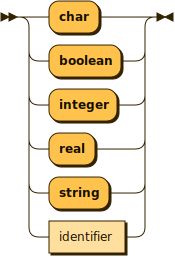
\includegraphics{diagram/typeid.pdf}

\end{figure}

\begin{grammarbox}[grammar:typeid]{typeid}
\vspace{0.5em}
typeid   ::= 'char'
           | 'boolean'
           | 'integer'
           | 'real'
           | 'string'
           | identifier
\end{grammarbox}

referenced by:

\begin{itemize}
\tightlist
\item
  \nameref{grammar:formal_parameter_section}
\item
  \nameref{grammar:proc_or_func}
\item
  \nameref{grammar:simple_type}
\item
  \nameref{grammar:tag_field}
\item
  \nameref{grammar:type}
\end{itemize}

\textbf{unsigned\_integer:}

\begin{figure}[H]
\centering
\includegraphics{diagram/unsigned_integer.pdf}

\end{figure}

\begin{grammarbox}[grammar:unsigned_integer]{unsigned\_integer}
\vspace{0.5em}
unsigned\_integer
         ::= INTEGER\_LITERAL
\end{grammarbox}

referenced by:

\begin{itemize}
\tightlist
\item
  \nameref{grammar:block}
\item
  \nameref{grammar:primary_expression}
\end{itemize}

\textbf{unsigned\_real:}

\begin{figure}[H]
\centering
\includegraphics{diagram/unsigned_real.pdf}

\end{figure}

\begin{grammarbox}[grammar:unsigned_real]{unsigned\_real}
\vspace{0.5em}
unsigned\_real
         ::= REAL\_LITERAL
\end{grammarbox}

referenced by:

\begin{itemize}
\tightlist
\item
  \nameref{grammar:primary_expression}
\end{itemize}

\textbf{integer\_literal:}

\begin{figure}[H]
\centering
\includegraphics{diagram/integer_literal.pdf}

\end{figure}

\begin{grammarbox}[grammar:integer_literal]{integer\_literal}
\vspace{0.5em}
integer\_literal
         ::= INTEGER\_LITERAL
\end{grammarbox}

referenced by:

\begin{itemize}
\tightlist
\item
  \nameref{grammar:constant}
\end{itemize}

\textbf{real\_literal:}

\begin{figure}[H]
\centering
\includegraphics{diagram/real_literal.pdf}

\end{figure}

\begin{grammarbox}[grammar:real_literal]{real\_literal}
\vspace{0.5em}
real\_literal
         ::= REAL\_LITERAL
\end{grammarbox}

referenced by:

\begin{itemize}
\tightlist
\item
  \nameref{grammar:constant}
\end{itemize}

\textbf{string\_literal:}

\begin{figure}[H]
\centering
\includegraphics{diagram/string_literal.pdf}

\end{figure}

\begin{grammarbox}[grammar:string_literal]{string\_literal}
\vspace{0.5em}
string\_literal
         ::= STRING\_LITERAL
\end{grammarbox}

referenced by:

\begin{itemize}
\tightlist
\item
  \nameref{grammar:constant}
\item
  \nameref{grammar:primary_expression}
\end{itemize}

\textbf{char\_literal:}

\begin{figure}[H]
\centering
\includegraphics{diagram/char_literal.pdf}

\end{figure}

\begin{grammarbox}[grammar:char_literal]{char\_literal}
\vspace{0.5em}
char\_literal
         ::= CHAR\_LITERAL
\end{grammarbox}

\textbf{boolean\_literal:}

\begin{figure}[H]
\centering
\includegraphics{diagram/boolean_literal.pdf}

\end{figure}

\begin{grammarbox}[grammar:boolean_literal]{boolean\_literal}
\vspace{0.5em}
boolean\_literal
         ::= BOOLEAN\_LITERAL
\end{grammarbox}

\textbf{empty:}

\begin{figure}[H]
\centering
\includegraphics{diagram/empty.pdf}

\end{figure}

\begin{grammarbox}[grammar:empty]{empty}
\vspace{0.5em}
empty    ::=
\end{grammarbox}

referenced by:

\begin{itemize}
\tightlist
\item
  \nameref{grammar:other_statement}
\end{itemize}

\section{Conclusão}
Essa documentação descreve formalmente a gramática PascalM com precisão,
auxiliando no desenvolvimento de compiladores, interpretadores ou ferramentas
de análise estática.

\end{document}
